\section{Mobile applications}
In recent years mobile applications are becoming increasingly popular in many domains, such as business, health and entertainment. According to the 2015 mobile app report \cite{ComScore}, the time spent on mobile devices grew up from 51 percent in share spent time to a 62 percent, leaving the share spent time of desktop on a 38 percent and becoming the number one of digital media consumption in 2015. Also, the usage of apps which include health or tracking functions was unknown until 2014, when several apps experienced a huge grow of up to 922 percent each year. 

\subsection{Personal applications and new hardware capabilities}

Mobile devices have reached a point where their hardware capabilities are comparable to a desktop computer capabilities regarding their processing power and available RAM; furthermore, they provide added functions that are unimaginable for a desktop computer, such as GPS, accelerometer; and the ability to be carried throughout the day. This enables new ways of living and interacting with technology as well as bringing closer the idea of ubiquitous computing, "perhaps ubiquitous computing is already here, but took a form other than that which had been envisioned." \cite{Bell2007}. 

\begin{figure}[h]
\begin{adjustbox}{width=.4\textwidth,center=\textwidth}
  \centering
  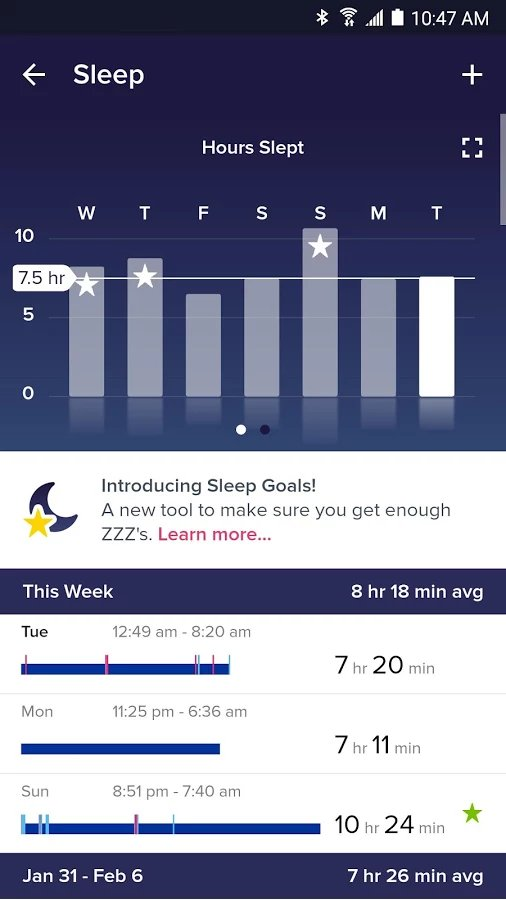
\includegraphics[scale=.5]{images/sleep_tracking.jpg}
\end{adjustbox}
  \caption[Fitbit application sleep tracking]{Fitbit application sleep tracking \footnote{\url{https://www.google.com/fit/}}}
  \label{fig:google_fit}
\end{figure}

Example of emerging applications that heavily rely on new devices hardware's capabilities, are Google Fit \footnote{\url{https://www.google.com/fit/}}, Nike + \footnote{\url{http://www.nike.com/us/en_us/c/nike-plus/running-app-gps}}, Fitbit \footnote{\url{https://www.fitbit.com/uk}} Jawbone Up \footnote{\url{https://jawbone.com/up}} and Garmin Connect \footnote{\url{https://connect.garmin.com/en-US/}}. These apps make use of sensors that although simple and cheap; are able to measure a range of activities carried out by a person. Such activities go from time and quality of sleep, calories ingested during the day, average heart rate of a run or steps taken during a city walk that according Morrison et al. \cite{Rooksby2014},  allows to count and measure areas of a person's life to optimize behavior as desired.

Recent research \cite{Barkhuus2011} suggests that people uses mobile applications in personalized or individual manners, adapting functions to meet their priorities; adding  new functions to create their own unique experiences based on their everyday lives. There is an enormous opportunity for crafting new applications that not only can give unique and valuable experiences; but influence the way people do things in the real world. 

\subsection{Challenges and usability considerations}

Core differences between desktop and mobile applications make mobile development more challenging than desktop development \cite{Chittaro2006}. Important examples of this that should be accounted when designing visualizations for mobile devices are, among others; limited processing power, smaller screen, multiple types of screens and slower connectivity. This issues become evident when trying to translate a visualization such as the shown in 
\iffalse
\ref{fig:web_based_desktop_visualization}, 
\begin{figure}[h]
\begin{adjustbox}{width=1.2\textwidth,center=\textwidth}
  \centering
  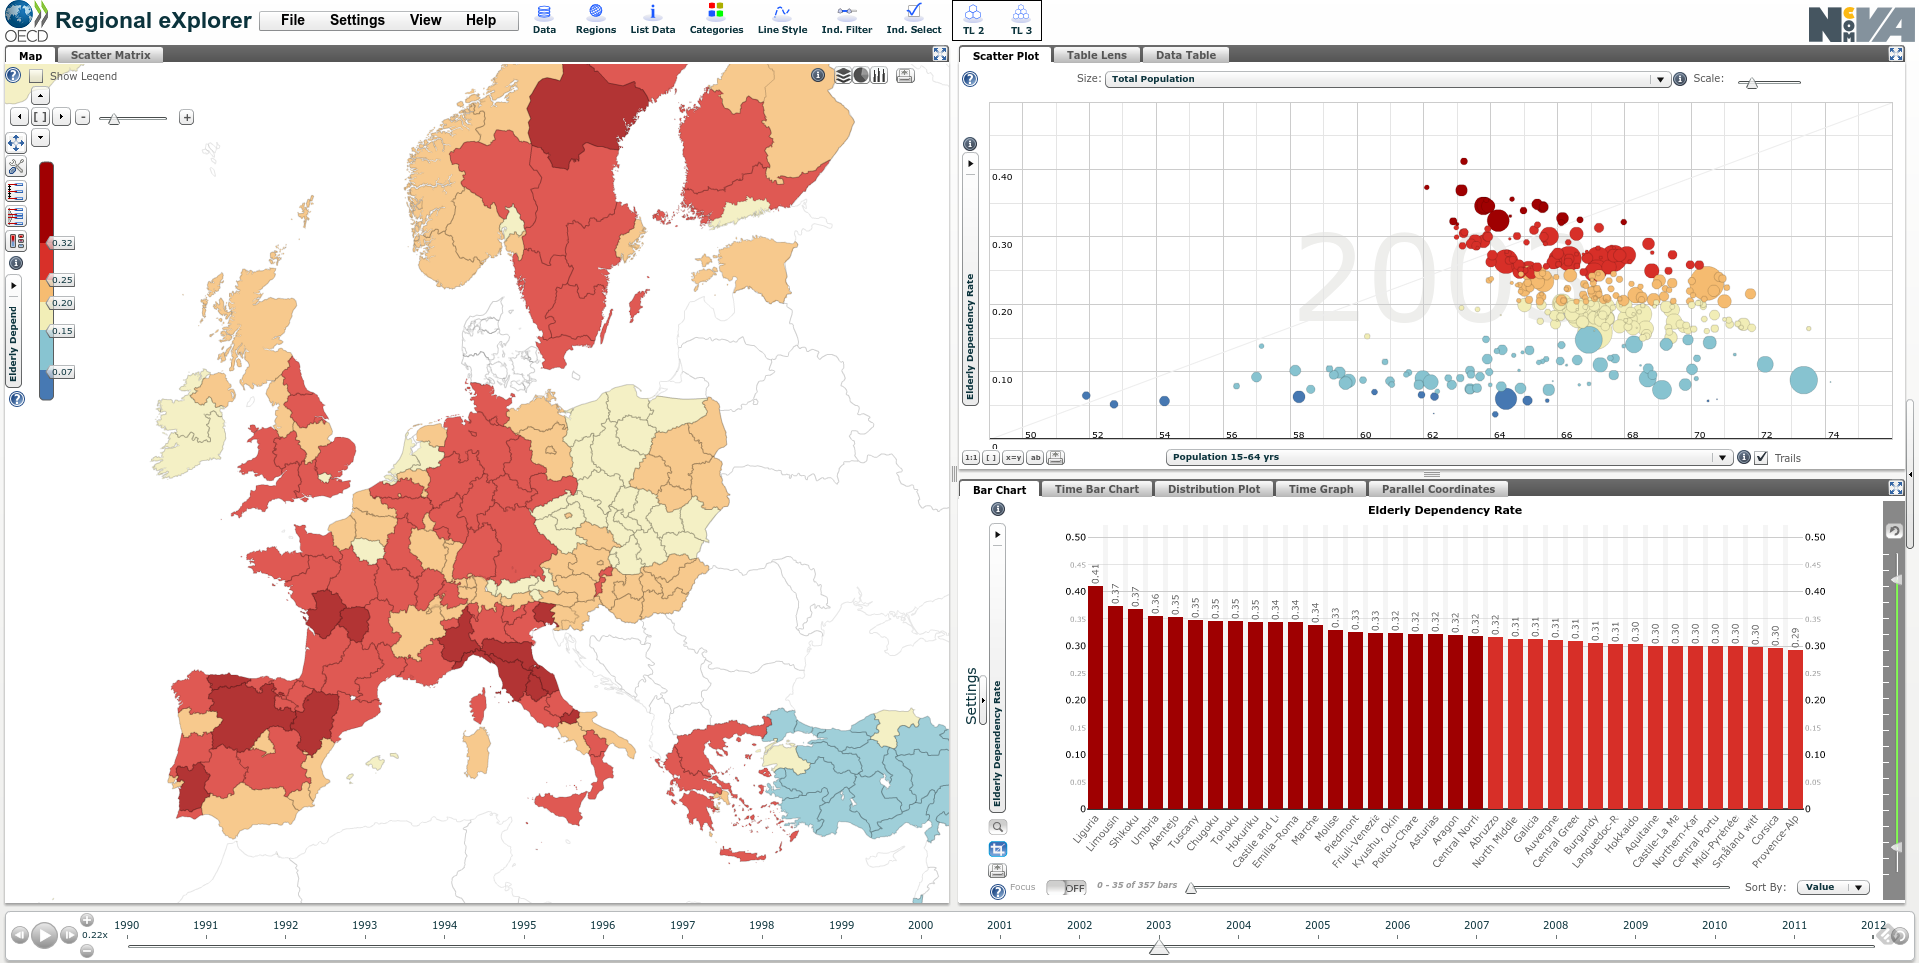
\includegraphics[scale=.5]{images/visualization_desktop_example.png}
\end{adjustbox}
  \caption[Line-based visualization]{Line-based visualization}
  \label{fig:web_based_desktop_visualization}
\end{figure}
\fi
It is particularly challenging to design mobile applications in contrast to desktop applications because 

(PEND)




